%
% Modo de operación CFB, capítulo de antecedentes.
% Proyecto Lovelace.
%

\subsection{\textit{Cipher Feedback} (CFB)}

Al igual que la operación de cifrado de CBC, ambas operaciones de CFB (cifrado
y descifrado) están encadenadas bloque a bloque, por lo que son de naturaleza
secuencial. En este caso, lo que se cifra en el primer paso es el vector de
inicialización; la salida de esto se opera con un \verb|xor| sobre el primer
bloque de texto en claro, para obtener el primer bloque cifrado (figura
\ref{fig:cfb}).

Esta distribución presenta varias ventajas con respecto a CBC: las operaciones
de cifrado y descifrado son sumamente similares, lo que permite ser
implementadas por un solo algoritmo (pseudocódigo \ref{cfb:1}); tanto para
cifrar como para descifrar solamente se ocupa la operación de cifrado del
algoritmo a bloques subyacente. Estas ventajas se deben principalmente a las
propiedades de la operación \verb|xor| (ecuación \ref{xor:inverso_igual}).

\begin{equation}
  \label{xor:inverso_igual}
  A \oplus B = C \quad \Rightarrow \quad A = B \oplus C
\end{equation}

\begin{figure}[H]
  \centering
  \begin{subfigure}{0.45\textwidth}
      \begin{center}
          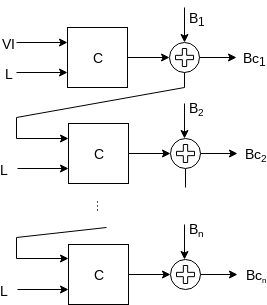
\includegraphics[width=0.6\linewidth]
            {contenidos/antecedentes/modos/diagramas/modo_cfb.png}
          \caption{Cifrado.}
      \end{center}
  \end{subfigure}
  \begin{subfigure}{0.45\textwidth}
      \begin{center}
          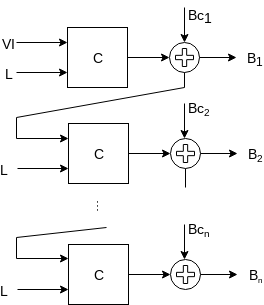
\includegraphics[width=0.6\linewidth]
            {contenidos/antecedentes/modos/diagramas/modo_cfb_inverso.png}
          \caption{Descifrado.}
      \end{center}
  \end{subfigure}
  \caption{Modo de operación CFB.}
  \label{fig:cfb}
\end{figure}

\begin{pseudocodigo}[caption={Modo de operación CFB (cifrado y descifrado).}, label={cfb:1}]
  entrada: llave $ L $; vector de inicialización $ VI $;
           bloques de mensaje (cifrado o descifrado) $ B_1, B_2 \dots B_n $.
   salida: bloques de mensaje (cifrado o descifrado) $ Bc_1, Bc_2 \dots Bc_n $.
  inicio
    $Bc_0$ $\gets$ $ VI $
    para_todo $B$
      $Bc_i$ $\gets$ C($L$, $Bc_{i - 1}$) $\oplus$ $B_i$
    fin
    regresar $Bc$
  fin
\end{pseudocodigo}
